% !TEX program = pdflatex
% Presentation superviseur -- Week 8 -- 2026-05-29
% Continuité Week 4 : roadmap globale, problèmes méthode + métrique,
% 3 sujets de travail S5-S8, méthodes nommées et résultats comparés.

\documentclass[aspectratio=169,10pt]{beamer}

\usepackage[utf8]{inputenc}
\usepackage[T1]{fontenc}
\usepackage[french]{babel}
\usepackage{lmodern}
\usepackage{booktabs}
\usepackage{array}
\usepackage{tikz}
\usepackage[table]{xcolor}
\usepackage{graphicx}
\usetikzlibrary{positioning, arrows.meta, shapes.geometric, fit, backgrounds, calc}

\usetheme{Madrid}
\usecolortheme{seahorse}
\setbeamertemplate{navigation symbols}{}
\setbeamertemplate{footline}[frame number]
\setbeamerfont{footnote}{size=\tiny}

\definecolor{accent}{RGB}{41, 92, 155}
\definecolor{accentsoft}{RGB}{230, 238, 247}
\definecolor{warn}{RGB}{200, 80, 40}
\definecolor{ok}{RGB}{30, 130, 70}
\definecolor{ppcol}{RGB}{47, 111, 79}
\definecolor{penalcol}{RGB}{124, 45, 45}
\definecolor{artcol}{RGB}{41, 92, 155}
\definecolor{jpcol}{RGB}{47, 111, 79}
\definecolor{crosscol}{RGB}{110, 60, 130}

\newcommand{\keybox}[1]{%
  \begin{center}
  \colorbox{accentsoft}{\parbox{0.92\linewidth}{\centering #1}}
  \end{center}}
\newcommand{\warnbox}[1]{%
  \begin{center}
  \colorbox{red!10}{\parbox{0.92\linewidth}{\centering #1}}
  \end{center}}
\newcommand{\okbox}[1]{%
  \begin{center}
  \colorbox{green!10}{\parbox{0.92\linewidth}{\centering #1}}
  \end{center}}
\newcommand{\crossbox}[1]{%
  \begin{center}
  \colorbox{violet!10}{\parbox{0.92\linewidth}{\centering #1}}
  \end{center}}

\title[KG juridique FR --- Week 8]{Construction d'un Knowledge Graph juridique français}
\subtitle{Point d'avancement --- Week 8 : nouveau benchmark, nouvelles méthodes, résultats comparés}
\author{Matthieu Kaeppelin}
\institute{Stage FE Recherche}
\date{29 mai 2026}

\begin{document}

% ============================================================
\begin{frame}
  \titlepage
\end{frame}

% ============================================================
\begin{frame}{Plan de la séance}
  \tableofcontents[hideallsubsections]
\end{frame}

% ============================================================
\section{Roadmap globale : d'où on part, où on va}

% ------- SLIDE ROADMAP ENRICHIE -------
\begin{frame}{Roadmap globale -- 15 paliers, état au 29 mai}
  \scriptsize
  \renewcommand{\arraystretch}{1.05}
  \begin{center}
  \begin{tabular}{@{}c p{8.5cm} l@{}}
    \toprule
    \textbf{\#} & \textbf{Palier} & \textbf{État} \\
    \midrule
    1  & Étude du state-of-the-art, papiers, fiches de lecture                        & \textcolor{ok}{\textbf{Validé S1--S2}} \\
    2  & Téléchargement des décisions Judilibre + étude de la donnée                  & \textcolor{ok}{\textbf{Validé S1--S2}} \\
    3  & Extraction des articles de loi (regex V5)                                    & \textcolor{ok}{\textbf{Validé S3}} \\
    4  & Construction graphe JP $\leftrightarrow$ Article + analyse macro            & \textcolor{ok}{\textbf{Validé S3}} \\
    5  & Construction d'un premier benchmark questions $\to$ article + JP (CRFPA 8 q) & \textcolor{ok}{\textbf{Validé S3--S4}} \\
    6  & Création des métriques d'évaluation                                          & \textcolor{ok}{\textbf{Validé S4 / raffiné S7}} \\
    7  & \textbf{Baseline 1} : embedding JP naïf -- mean pooling sur la JP entière    & \textcolor{warn}{\textbf{Échec démasqué S4}} \\
    \rowcolor{accentsoft}
    8  & Pivot \emph{articles-first} -- \textbf{Baseline 2} : embedding des articles  & \textcolor{ok}{\textbf{Validé S5--S7}} \\
    \rowcolor{accentsoft}
    9  & Construction de résumés / synthèses des JP (via DB OVH Hector)               & \textcolor{ok}{\textbf{Validé S7}} \\
    \rowcolor{accentsoft}
    10 & Embedding des résumés JP -- \textbf{Baseline 3}                              & \textcolor{ok}{\textbf{Validé S7--S8}} \\
    \rowcolor{accentsoft}
    11 & Agrandissement du benchmark pénal -- doctrine scrapée + qgen LLM            & \textcolor{accent}{\textbf{Validé S8}} \\
    \rowcolor{accentsoft}
    12 & Évaluation comparée des méthodes sur le gros benchmark                       & \textcolor{accent}{\textbf{Validé S8}} \\
    \rowcolor{accentsoft}
    13 & \textbf{Baseline 4} : stratégies cross-modales (2 espaces d'embedding)       & \textcolor{accent}{\textbf{Émerge S8}} \\
    14 & Construction d'un graphe pénal enrichi avec nœuds \og question \fg{}         & \textcolor{warn}{\textbf{À explorer S9+}} \\
    15 & GNN link prediction final                                                    & \textbf{Étape 3} \\
    \bottomrule
  \end{tabular}
  \end{center}
\end{frame}

% ============================================================
\section{Rappel du cadre de travail}

\begin{frame}{Rappel S4 : focus sur le sous-corpus pénal}
  \footnotesize
  Le corpus complet (1,07 M arrêts) est trop gros pour itérer rapidement.
  \textbf{Sous-graphe thématique} : toute JP citant au moins un article d'un \textbf{code pénal}.

  \vspace{0.4em}
  \textbf{Filtre} : codes \texttt{penal} (2 999 art.), \texttt{procedure\_penale} (3 924),
  \texttt{route} (1 125), \texttt{justice\_penale\_mineurs} (37).

  \vspace{0.6em}
  \renewcommand{\arraystretch}{1.2}
  \begin{center}
  \begin{tabular}{@{}l r r@{}}
    \toprule
     & \textbf{Corpus complet} & \textbf{Sous-corpus pénal} \\
    \midrule
    JP totales      & 1 072 646 & \textbf{118 112} \\
    \quad Cour de cassation       & 511 575   & 97 060 \\
    \quad Cours d'appel           & 422 965   & 14 315 \\
    \quad Tribunaux judiciaires   & 138 106   & 6 737 \\
    Articles cités (graphe)       & 87 821    & 87 821 \\
    Citations totales (arêtes)    & 6 444 358 & 2 026 258 (pénal-side) \\
    Questions CRFPA évaluables    & 41        & \textbf{8} \\
    \bottomrule
  \end{tabular}
  \end{center}

  \vspace{0.5em}
  \keybox{Tout le reste de la présentation se place dans ce cadre $\to$
  \textbf{8 questions pénales, 118 k JP, 87 k articles}.}
\end{frame}

\begin{frame}{Le graphe biparti article $\leftrightarrow$ JP}
  \footnotesize
  \textbf{Structure} : graphe biparti non orienté où chaque arête « JP cite article ».

  \vspace{0.3em}
  \begin{columns}[T]
    \column{0.55\textwidth}
    \centering
    \begin{tikzpicture}[node distance=0.7em,
      art/.style={circle, draw=artcol, fill=artcol!15, minimum size=0.7cm, font=\tiny\bfseries},
      jp/.style={rectangle, draw=jpcol, fill=jpcol!15, rounded corners=2pt, minimum width=1.4cm, minimum height=0.5cm, font=\tiny},
      edge/.style={-, gray!60, thin}]

      % Colonne articles (gauche)
      \node[art] (a1) at (0, 3)   {A1};
      \node[art] (a2) at (0, 2.2) {A2};
      \node[art] (a3) at (0, 1.4) {A3};
      \node[art] (a4) at (0, 0.6) {A4};
      \node[art] (a5) at (0, -0.2) {A5};
      \node[at={(0,-0.9)}, font=\tiny\bfseries\color{artcol}] {\ldots 87 821 articles};

      % Colonne JP (droite)
      \node[jp] (j1) at (4, 3.2)  {JP$_1$ -- CC};
      \node[jp] (j2) at (4, 2.4)  {JP$_2$ -- CA};
      \node[jp] (j3) at (4, 1.6)  {JP$_3$ -- CC};
      \node[jp] (j4) at (4, 0.8)  {JP$_4$ -- TJ};
      \node[jp] (j5) at (4, 0)    {JP$_5$ -- CC};
      \node[jp] (j6) at (4, -0.8) {JP$_6$ -- CA};
      \node[at={(4,-1.5)}, font=\tiny\bfseries\color{jpcol}] {\ldots 118 112 JP pénales};

      % Aretes
      \draw[edge] (a1) -- (j1);
      \draw[edge] (a1) -- (j3);
      \draw[edge] (a2) -- (j1);
      \draw[edge] (a2) -- (j2);
      \draw[edge] (a2) -- (j5);
      \draw[edge] (a3) -- (j2);
      \draw[edge] (a3) -- (j4);
      \draw[edge] (a3) -- (j6);
      \draw[edge] (a4) -- (j3);
      \draw[edge] (a4) -- (j5);
      \draw[edge] (a4) -- (j6);
      \draw[edge] (a5) -- (j4);
      \draw[edge] (a5) -- (j5);

      \node[at={(2,3.8)}, font=\tiny\itshape\color{gray!70}] {citations (regex V5)};
    \end{tikzpicture}

    \column{0.43\textwidth}
    \renewcommand{\arraystretch}{1.3}
    \begin{tabular}{@{}l r@{}}
      \toprule
      \textbf{Composante} & \textbf{Valeur} \\
      \midrule
      Nœuds \texttt{Article}  & 87 821 \\
      Nœuds \texttt{JP} (pénal) & 118 112 \\
      Arêtes (citations)      & 2 026 258 \\
      Composantes connexes    & \textbf{99,88 \% en 1 seule} \\
      \bottomrule
    \end{tabular}

    \vspace{0.5em}
    \scriptsize
    \keybox{Structure exploitable : connexe, très concentrée sur des articles-piliers, propice au back-edge.}
  \end{columns}
\end{frame}

\begin{frame}{Les 8 questions pénales du benchmark CRFPA}
  \footnotesize
  Sur les 41 questions du benchmark CRFPA (CNB 2025), \textbf{8 sont pénales} :
  3 droit pénal + 5 procédure pénale.

  \vspace{0.4em}
  \renewcommand{\arraystretch}{1.2}
  \begin{center}
  \begin{tabular}{@{}l p{6.8cm} c c@{}}
    \toprule
    \textbf{ID} & \textbf{Thème} & \textbf{N art} & \textbf{N JP} \\
    \midrule
    \texttt{PENAL-Q1} & Infractions sexuelles (viol conjugal) + irresponsabilité          & 14 & 7 \\
    \texttt{PENAL-Q2} & Infractions non intentionnelles (blessures involontaires)         &  5 & 2 \\
    \texttt{PENAL-Q3} & Responsabilité pénale des personnes morales                       &  3 & 4 \\
    \texttt{PP-Q1}    & Mesures d'investigation : géolocalisation                         &  6 & 2 \\
    \texttt{PP-Q2}    & Garde à vue : régularité du placement                             &  5 & 3 \\
    \texttt{PP-Q3}    & Interrogatoire de première comparution                            &  4 & 3 \\
    \texttt{PP-Q4}    & Qualité à agir et délai sur nullités                              &  5 & 3 \\
    \texttt{PP-Q5}    & Détention provisoire : assistance obligatoire                     &  9 & 0 \\
    \midrule
    \textbf{Total} & & \textbf{51} & \textbf{24} \\
    \bottomrule
  \end{tabular}
  \end{center}

  \vspace{0.4em}
  \textbf{Gold attendu par question} : un set d'articles obligatoires +
  un set de JP de référence (pourvois CC).
\end{frame}

% ============================================================
\section{Les deux problèmes diagnostiqués en S4}

\begin{frame}{Problème 1 -- la méthode d'embedding était cassée}
  \footnotesize
  \textbf{Setup palier 7 -- Baseline 1} :
  encoder \texttt{multilingual-e5-base} (768d, contexte 512 tok) sur les
  \textbf{118 112 JP pénales entières}, chunk de 510 tokens avec overlap 64,
  \textbf{cap à 8 chunks} par doc, \textbf{mean pooling} $\to$ 1 vecteur par JP.
  \\
  \emph{Note} : appelée \og B2 \fg{} en S4 (« 2\textsuperscript{e} baseline » testée), devient \textbf{Baseline 1} dans la chronologie globale.

  \vspace{0.5em}
  \textbf{Symptômes observés} (audit post-run) :

  \vspace{0.3em}
  \scriptsize
  \renewcommand{\arraystretch}{1.2}
  \begin{columns}[T]
    \column{0.48\textwidth}
    \centering
    \textbf{Côté JP -- top-K direct}\\[0.3em]
    \begin{tabular}{@{}l r@{\hspace{0.8em}} l r@{}}
      \toprule
      \textbf{Métrique} & \textbf{Valeur} & \textbf{Recall GT} & \textbf{Rés.}\\
      \midrule
      Rang médian GT JP & \textbf{76 782} & top-10     & 0 / 16 \\
      Rang moyen GT     & 58 319          & top-100    & 0 / 16 \\
                        &                 & top-1 000  & 2 / 16 \\
                        &                 & top-10 000 & 3 / 16 \\
      \bottomrule
    \end{tabular}

    \column{0.48\textwidth}
    \centering
    \textbf{Côté articles -- via 1-hop graphe}\\[0.3em]
    \begin{tabular}{@{}l r r r@{}}
      \toprule
      \textbf{Stratégie} & \textbf{Recall} & \textbf{n\_ret.} & \textbf{Préc.}\\
      \midrule
      union K=5             & 0,182       & 31   & 3,7 \% \\
      union K=10 (baseline) & 0,315       & 49   & 3,7 \% \\
      union K=20 (extrap.)  & $\sim$0,45  & $\sim$90 & $\sim$3,2 \% \\
      \bottomrule
    \end{tabular}\\[0.4em]
    \textit{\scriptsize Recall articles atteint 0,315 mais au prix de 49 articles retournés (précision 3,7 \%) -- score gonflé par over-retrieval, pas exploitable en production.}
  \end{columns}

  \vspace{0.4em}
  \warnbox{\textbf{Aucune référence pertinente n'apparaît avant le rang 549.}
  L'embedding ne capture quasiment aucun signal -- ni l'encodeur (e5-base
  non spécialisé juridique), ni le \emph{mean pooling sur 8 chunks} qui dilue
  le passage discriminant dans le boilerplate (faits, formules, procédure).}
\end{frame}

\begin{frame}{Problème 2 -- la métrique était aussi cassée}
  \footnotesize
  \textbf{Métrique palier 6 (v1) -- score CRFPA} :
  \[ S_{\text{retrieval}} = 0{,}5 \cdot \bar{S}_{\text{art}} + 0{,}5 \cdot \bar{S}_{\text{jp}}
   \quad \text{(somme pondérée des recall pondérés par strate)} \]

  \vspace{0.5em}
  \textbf{Pourquoi c'est insuffisant} : multi-hop sur le graphe permet de
  \og gagner \fg{} le score en remontant simplement plus d'articles.

  \vspace{0.3em}
  \renewcommand{\arraystretch}{1.2}
  \begin{center}
  \begin{tabular}{@{}l r r r@{}}
    \toprule
    \textbf{Configuration} & \textbf{$\bar{S}_{\text{art}}$} & \textbf{Articles retournés} & \textbf{Précision} \\
    \midrule
    \texttt{1-hop} (baseline B2)   & 0,315          & 49    & 3,67 \% \\
    \texttt{2-hop M=2}             & \textbf{0,893} & 9 189 & \textcolor{warn}{\textbf{0,06 \%}} \\
    \texttt{2-hop M=3}             & 0,794          & 5 028 & 0,12 \% \\
    \bottomrule
  \end{tabular}
  \end{center}

  \vspace{0.5em}
  \warnbox{\textbf{Recall 89 \% pour une précision 0,06 \%} -- on retourne 9 189
  articles pour récupérer le gold. \textbf{Pas exploitable en pratique.}
  La métrique récompense le sur-pêchage et ne mesure pas la qualité réelle du retrieval.}

  \vspace{0.4em}
  $\Rightarrow$ Sans précision implicite, on ne peut pas distinguer un système qui
  trouve 1 article pertinent dans le top-10 d'un système qui en trouve 1 dans le top-10 000.
\end{frame}

\begin{frame}{Métrique adoptée à partir de S7 (palier 6, v2)}
  \footnotesize
  \textbf{Métrique principale} -- on regarde directement deux valeurs :

  \vspace{0.5em}
  \begin{center}
  \renewcommand{\arraystretch}{1.4}
  \begin{tabular}{@{}p{4cm} p{8cm}@{}}
    \toprule
    \textbf{Côté articles} & \texttt{recall@10} sur le gold des articles obligatoires \\
    \textbf{Côté JP}       & \texttt{recall@5} sur le gold des pourvois CC \\
    \bottomrule
  \end{tabular}
  \end{center}

  \vspace{0.5em}
  \textbf{Lecture} : on compare directement les valeurs de recall et de précision entre méthodes -- la méthode qui maximise les deux pour un même $K$ gagne.
  Pour la robustesse \emph{par question}, on rapporte aussi le nombre de questions atteignant
  $\geq 0{,}5$ ou $\geq 0{,}8$ de recall (indicateurs secondaires).

  \vspace{0.5em}
  \textbf{Pourquoi ces $K$} : recall@10 articles borne implicitement la précision (pour 1 article gold, précision max 10 \% ; pour 7 articles, précision max 70 \%). recall@5 JP est plus serré car les questions ont souvent peu de JP gold.

  \vspace{0.5em}
  \keybox{Cette métrique remplace le \(S_{\text{retrieval}}\) du S4 qui pouvait être gonflé par le sur-pêchage (recall 89 \% avec 9 189 articles retournés). \textbf{Ajout S8} : on suit désormais aussi la précision \emph{moyenne} pour ne plus se laisser tromper par les méthodes set qui retournent des centaines de candidats.}
\end{frame}

\begin{frame}{Reformulation S9 (point Johnny du 29/05)}
  \scriptsize
  \textbf{Défaut identifié} : pour les variantes set (B4-a union, B4-b intersection),
  le rappel naïf $|R \cap S|/|R|$ était calculé sur un $S$ de taille \emph{variable} entre
  méthodes ($|S|=730$ pour B4-a, $|S|=2$ pour B4-b). Méthodes incomparables.

  \vspace{0.4em}
  \textbf{Définition propre} -- procédure uniforme pour toutes les méthodes :

  \vspace{0.3em}
  \begin{enumerate}\setlength\itemsep{0.15em}
    \item La méthode $\mathcal{M}$ produit $S = \mathcal{M}(Q_a)$, $|S| = p$
    \item $Z_i = \cos(X_{Q_a},\, X_{S_i})$ pour $i \in S$
    \item $\text{rank}(Z, K) = $ les $K$ candidats de $S$ de plus haute similarité cosinus
    \item $\text{recall@K} = \dfrac{|R_{Q_a} \cap \text{rank}(Z, K)|}{|R_{Q_a}|}
           \qquad \text{precision@K} = \dfrac{|R_{Q_a} \cap \text{rank}(Z, K)|}{K}$
  \end{enumerate}

  \vspace{0.4em}
  \begin{center}
  \renewcommand{\arraystretch}{1.2}
  \begin{tabular}{@{}l c c@{}}
    \toprule
    \textbf{Paramètre} & \textbf{Articles} & \textbf{JP} \\
    \midrule
    $K_{\text{final}}$ rapporté & 10 et 20 & 5 et 10 \\
    $K_{\text{in}}$ (construction de $S$) & 10, 20, 50 & 10, 20, 50 \\
    Distance & cosinus sur BGE-M3 normalisé & idem \\
    \bottomrule
  \end{tabular}
  \end{center}

  \vspace{0.3em}
  \keybox{$K$ devient un \textbf{budget de lecture fixe}, identique entre toutes les méthodes.
  Les méthodes set ne peuvent plus tricher : un $S$ large ne donne plus un rappel artificiel
  si son ranking interne est mauvais.}

  \vspace{0.3em}
  \textbf{Définition complémentaire -- gold étendu} : $R^{\text{art-ext}}_{Q_a} = R^{\text{art}}_{Q_a} \cup \{$articles cités par les JP de $R^{\text{jp}}_{Q_a}$ via le graphe$\}$. Médiane $|R^{\text{art}}|$ passe de 1 à 3 $\to$ précision plafond de 10 \% à 30 \% à $K{=}10$.
\end{frame}

\begin{frame}{Distribution du gold attendu par question (strict + étendu)}
  \scriptsize
  \centering
  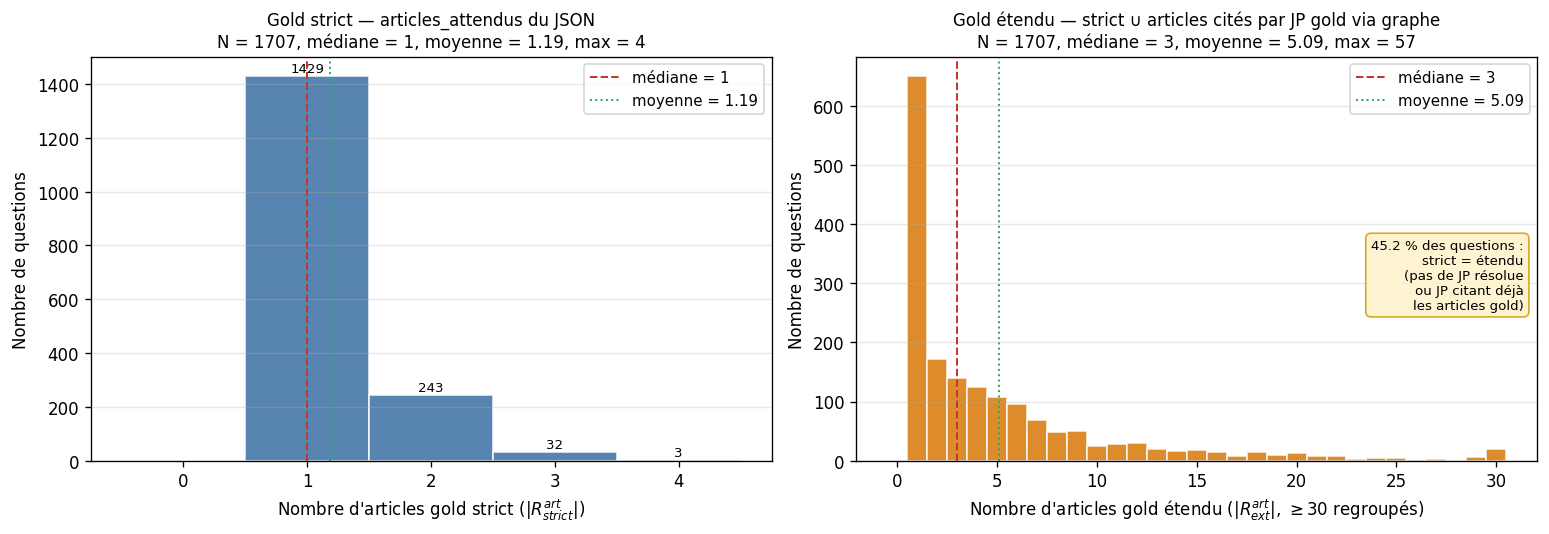
\includegraphics[width=0.98\linewidth]{../../05-Technique/benchmark/etape1_embedding_pur/data/doctrine_qgen/fig_gold_size_articles}

  \vspace{0.3em}
  \begin{columns}[T]
    \column{0.50\textwidth}
    \footnotesize\textbf{Articles strict} ($N = 1\,707$)
    \begin{itemize}\setlength\itemsep{0pt}
      \item médiane $= 1$, moyenne $= 1{,}19$, max $= 4$
      \item \textbf{83,7 \%} des questions ont \textbf{1 seul} article gold
    \end{itemize}
    \footnotesize\textbf{Articles étendu} ($\cup$ articles cités par JP gold)
    \begin{itemize}\setlength\itemsep{0pt}
      \item médiane $= 3$, moyenne $= 5{,}09$, max $= 57$
      \item $54{,}8$ \% gagnent $\geq 1$ article via les JP
    \end{itemize}

    \column{0.50\textwidth}
    \footnotesize\textbf{JP CC résolues} ($N = 1\,707$)
    \begin{itemize}\setlength\itemsep{0pt}
      \item médiane $= 1$, moyenne $= 0{,}65$, max $= 4$
      \item \textbf{43,1 \%} des questions ont 0 JP résolue
      \item $971 / 1\,707$ questions ont $\geq 1$ JP
    \end{itemize}
    \footnotesize\textbf{Pas d'extension du gold JP}
    \begin{itemize}\setlength\itemsep{0pt}
      \item Extension via articles citants $\to$ circulaire pour B3-b
    \end{itemize}
  \end{columns}

  \vspace{0.2em}
  \warnbox{\textbf{Plafond mécanique de la précision} -- strict : $1/K$ pour la médiane $|R|{=}1$
  (10 \% à $K{=}10$, 5 \% à $K{=}20$). Étendu : $3/K$ pour la médiane $|R|{=}3$ (30 \% à $K{=}10$).
  Les chiffres de précision deviennent interprétables sous le gold étendu.}
\end{frame}

% ============================================================
\section{Trois sujets de travail depuis Week 4}

\begin{frame}{Vue d'ensemble des 3 chantiers menés en parallèle}
  \footnotesize
  \begin{enumerate}\setlength\itemsep{0.6em}
    \item \textbf{Changer ce qu'on embed} \hfill (paliers \textbf{8}, \textbf{9}, \textbf{10})
    \\ Constat palier 7 : embedder les JP entières + mean pooling = signal cassé.
    \\ Plusieurs options : \emph{Baseline 2} (articles), complétion par optimisation, \emph{Baseline 3} (synthèses LLM).

    \item \textbf{Augmenter le benchmark} \hfill (palier \textbf{11})
    \\ Le benchmark CRFPA = 8 questions pénales seulement. Trop peu pour stratifier.
    \\ $\to$ Scrapping de doctrine (Jurisclasseurs LexisNexis) + génération de questions par LLM.

    \item \textbf{Enrichir le graphe avec des nœuds \og question \fg} \hfill (palier \textbf{14})
    \\ Une fois qu'on a beaucoup de questions étiquetées (gold articles + JP),
    on peut les ajouter au graphe et faire du \emph{link prediction} via GNN.
  \end{enumerate}
\end{frame}

% ============================================================
\subsection{Chantier 1 -- changement du point d'entrée d'embedding (paliers 8--10)}

\begin{frame}{Chantier 1 -- de quoi on part, où on va}
  \footnotesize
  \textbf{Constat palier 7 (Baseline 1)} : embedder les \textbf{JP entières} +
  \textbf{mean pooling sur 8 chunks} produit un signal cassé
  (rang médian gold = 76 782 / 118 112).

  \vspace{0.4em}
  \textbf{Trois pistes pour reconstruire un signal exploitable} :

  \vspace{0.5em}
  \renewcommand{\arraystretch}{1.4}
  \begin{tabular}{@{}c p{4.6cm} p{6.0cm}@{}}
    \toprule
    \textbf{Piste} & \textbf{Idée} & \textbf{Statut} \\
    \midrule
    \textbf{(a)} & Embedder les \textbf{articles de loi} au lieu des JP
    -- $\to$ \textbf{Baseline 2} (palier 8) &
    \textcolor{ok}{\textbf{Adopté S5--S7}} -- articles courts, knowledge concentré,
    pivot du point d'entrée. \\
    \midrule
    \textbf{(b)} & \textbf{Recompute les résumés JP par optimisation} (laplacien)
    sur le graphe & \textcolor{warn}{\textbf{Écarté}} -- méthode élégante mais
    données trop sparses, peu efficace en pratique. \\
    \midrule
    \textbf{(c)} & \textbf{Recréer des résumés / synthèses LLM} des JP (palier 9)
    puis embedder -- $\to$ \textbf{Baseline 3} (palier 10) &
    \textcolor{ok}{\textbf{Adopté S7--S8}} -- via calcul de plusieurs champs
    d'analyse de la JP (\texttt{step1\_raw}, 10 champs dont une synthèse pour avocat),
    produit sur le cluster Hector. \\
    \bottomrule
  \end{tabular}

  \vspace{0.4em}
  \keybox{\textbf{Conséquence structurelle} : on a maintenant \textbf{deux espaces d'embedding
  indépendants} -- articles (BGE-M3 sur texte LEGI) et synthèses JP (BGE-M3 sur synthèses LLM).
  $\to$ rend possible la \textbf{Baseline 4} (palier 13, cross-modale).}
\end{frame}

% ============================================================
\subsection{Chantier 2 -- agrandissement du benchmark (palier 11)}

\begin{frame}{Chantier 2 -- pipeline doctrine\_qgen}
  \footnotesize
  \textbf{Source} : 230 fascicules \emph{Jurisclasseurs procédure pénale} (LexisNexis),
  5 990 pages au total. Scrapping + parsing PDF.

  \vspace{0.4em}
  \textbf{Pipeline 4 phases} :
  \begin{enumerate}\setlength\itemsep{0.2em}
    \item Parsing PDF $\to$ sections JSON + whitelists d'articles/JP par sous-section
    \item Génération par LLM (Gemma 4 26B-A4B, vLLM, JSON schema strict) $\to$ question + gold
    \item Validation déterministe : articles cités $\subseteq$ whitelist, JP citées $\subseteq$ whitelist
    \item Anonymisation A/B pour revue humaine
  \end{enumerate}

  \vspace{0.4em}
  \renewcommand{\arraystretch}{1.2}
  \begin{center}
  \begin{tabular}{@{}l r@{}}
    \toprule
    \textbf{Métrique} & \textbf{Valeur} \\
    \midrule
    Documents JSON sections L1                         & 230 \\
    Sections L1 distinctes                              & 792 \\
    Articles cités distincts (whitelist)                & 18 447 \\
    JP citées distinctes (whitelist)                    & 33 421 \\
    \textbf{Questions clean générées}                   & \textbf{3 421} \\
    \quad dont strict (article \emph{ET} JP comme gold) & \textbf{1 707} ($\times$213 vs CRFPA pénal) \\
    Hallucinations détectées (sample review 20 q)       & 0 \\
    \bottomrule
  \end{tabular}
  \end{center}

  \vspace{0.4em}
  \okbox{Pipeline branche-agnostique : extensible à civil / admin / social en fournissant les Jurisclasseurs correspondants.}
\end{frame}

% ============================================================
\section{Méthodes testées et résultats comparés}

\begin{frame}{Méthodes testées -- classification par baseline}
  \scriptsize

  \renewcommand{\arraystretch}{1.2}
  \begin{tabular}{@{}l l p{8.5cm}@{}}
    \toprule
    \textbf{Baseline} & \textbf{Variante} & \textbf{Définition} \\
    \midrule
    \multicolumn{3}{@{}l@{}}{\textit{\textbf{Baseline 1} (palier 7) -- embedding JP entières + mean pooling}} \\
    B1 & --                  & \texttt{multilingual-e5-base} sur JP entières $\to$ rang médian gold = 76 782 \\
    \midrule
    \multicolumn{3}{@{}l@{}}{\textit{\textbf{Baseline 2} (palier 8) -- embedding des articles}} \\
    B2-a & cosine ouvert      & top-$K$ articles, pool 31 357 articles tous codes \\
    B2-b & cosine filtré      & top-$K$ articles, pool 3 603 articles (4 codes pénal) \\
    \midrule
    \multicolumn{3}{@{}l@{}}{\textit{\textbf{Baseline 3} (palier 10) -- embedding des synthèses LLM des JP}} \\
    B3-a & cosine direct      & top-$K$ JP par cosine sur \texttt{emb\_jp\_synthese} (116 755 JP) \\
    B3-b & Art $\to$ JP union & top-$K$ articles (B2) $\to$ union des JP citantes via graphe \\
    B3-c & Art $\to$ JP inter & top-$K$ articles (B2) $\to$ JP citant \emph{tous} ces articles \\
    B3-d & Art $\to$ JP maj.  & top-$K$ articles (B2) $\to$ JP citant $\geq \lceil K/2 \rceil$ \\
    B3-e & JP $\to$ Art union & top-$K$ JP (B3-a) $\to$ union des articles cités via graphe \\
    \midrule
    \multicolumn{3}{@{}l@{}}{\textit{\textbf{Baseline 4} (palier 13) -- cross-modal : combinaison des 2 espaces d'embedding}} \\
    B4-a & cross-union art    & articles top-$K$ B2 $\cup$ articles top-$K$ B3-e \\
    B4-b & cross-inter art    & articles top-$K$ B2 $\cap$ articles top-$K$ B3-e \\
    B4-c & cross-union JP     & JP top-$K$ B3-a $\cup$ JP top-$K$ B3-b \\
    B4-d & cross-inter JP     & JP top-$K$ B3-a $\cap$ JP top-$K$ B3-b \\
    \bottomrule
  \end{tabular}

  \vspace{0.4em}
  \keybox{\textbf{Côté articles} : 2 variantes B2 + 1 variante B3-e + 2 variantes B4 = 5 méthodes.
  \textbf{Côté JP} : 1 variante B3-a + 3 variantes B3-b/c/d + 2 variantes B4 = 6 méthodes.}
\end{frame}

\begin{frame}{Résultats côté ARTICLES -- métrique S9 (strict + gold étendu)}
  \tiny
  \textit{Gold \textbf{strict} = \texttt{articles\_attendus} du JSON. \quad
  Gold \textbf{étendu} = strict $\cup$ articles cités par les JP gold via graphe
  (médiane $|R|$ : strict = 1, étendu = 3). \quad
  Tous chiffres après re-rank cosinus puis cut à $K$.}

  \vspace{0.3em}
  \scriptsize
  \renewcommand{\arraystretch}{1.05}
  \setlength{\tabcolsep}{3pt}
  \begin{center}
  \begin{tabular}{@{}l l c c r | r r | r r@{}}
    \toprule
    & & & & & \multicolumn{2}{c|}{\textbf{Gold strict}} & \multicolumn{2}{c}{\textbf{Gold étendu}} \\
    \textbf{Var.} & \textbf{Méthode}
    & $K_{\text{in}}$ & $K$ & $|S|$ moy.
    & \textbf{Rec.} & \textbf{Préc.}
    & \textbf{Rec.} & \textbf{Préc.} \\
    \midrule
    B2-a & cosine art. pool ouvert        & -- & 10 & 31 357 & 0,450 & 5,1 \% & 0,294 & 7,5 \% \\
    B2-a & cosine art. pool ouvert        & -- & 20 & 31 357 & 0,538 & 3,1 \% & 0,354 & 4,7 \% \\
    B2-b & cosine art. pool pénal strict  & -- & 10 & 3 603  & 0,490 & 5,6 \% & 0,317 & 8,3 \% \\
    B2-b & cosine art. pool pénal strict  & -- & 20 & 3 603  & 0,582 & 3,4 \% & 0,384 & 5,4 \% \\
    \midrule
    \rowcolor{accentsoft}
    B3-e & JP $\to$ Art via graphe        & 10 & 10 & 30,8   & \textbf{0,656} & \textbf{7,7 \%} & \textbf{0,474} & \textbf{15,5 \%} \\
    \rowcolor{accentsoft}
    B3-e & JP $\to$ Art via graphe        & 10 & 20 & 30,8   & 0,709 & 4,2 \% & 0,581 & 11,1 \% \\
    B3-e & JP $\to$ Art via graphe        & 20 & 10 & 52,3   & 0,643 & 7,5 \% & 0,450 & 14,0 \% \\
    \rowcolor{accentsoft}
    B3-e & JP $\to$ Art via graphe        & 20 & 20 & 52,3   & \textbf{0,719} & 4,2 \% & \textbf{0,554} & 9,7 \% \\
    \midrule
    B4-a & cross-union art.               & 10 & 10 & 38,9   & \textcolor{warn}{0,450} & 5,1 \% & 0,294 & 7,5 \% \\
    B4-a & cross-union art.               & 10 & 20 & 38,9   & 0,746 & 4,4 \% & 0,558 & 9,2 \% \\
    \midrule
    B4-b & cross-inter art.               & 10 & 10 & 1,9    & 0,375 & 4,3 \% & 0,235 & 6,1 \% \\
    B4-b & cross-inter art.               & 50 & 10 & 8,8    & 0,568 & 6,6 \% & 0,381 & \textbf{10,8 \%} \\
    B4-b & cross-inter art.               & 50 & 20 & 8,8    & 0,578 & 3,3 \% & 0,392 & 5,7 \% \\
    \bottomrule
  \end{tabular}
  \end{center}

  \vspace{0.2em}
  \okbox{\textbf{B3-e domine sur les deux métriques} : strict (recall $0{,}66$, prec $7{,}7$ \%)
  et étendu (recall $0{,}47$, prec \textbf{$15{,}5$ \%}). Sous gold étendu, la précision plafond passe
  de $10$ \% (médiane $|R|=1$) à $30$ \% (médiane $|R|=3$). \textbf{Le classement est invariant} :
  B3-e $>$ B4-b $>$ B2-b. Avantage circulaire de B3-e à noter (son $S$ vient des JP citantes).}
\end{frame}

\begin{frame}{Résultats côté JP -- 971 questions, métrique S9}
  \tiny
  \textit{Évaluable JP = gold résolvable par regex pourvoi CC ($971/1\,707$).
  Tous les chiffres après \textbf{re-rank cosinus} de $S$ puis cut à $K_{\text{final}}$.}

  \vspace{0.3em}
  \scriptsize
  \renewcommand{\arraystretch}{1.1}
  \setlength{\tabcolsep}{3pt}
  \begin{center}
  \begin{tabular}{@{}l l c c r r r r@{}}
    \toprule
    \textbf{Var.} & \textbf{Méthode}
    & $K_{\text{in}}$ & $K_{\text{fin.}}$ & $|S|$ moy.
    & \textbf{Recall} & \textbf{Précision} & \textbf{\# q $r\geq 0{,}5$} \\
    \midrule
    \rowcolor{accentsoft}
    B3-a & cosine direct synthèses JP    & -- &  5 & 116 755 & \textbf{0,345} & \textbf{7,4 \%} & \textbf{35,7 \%} \\
    \rowcolor{accentsoft}
    B3-a & cosine direct synthèses JP    & -- & 10 & 116 755 & \textbf{0,406} & 4,4 \% & \textbf{42,1 \%} \\
    \midrule
    B3-b & Art $\to$ JP via graphe       & 10 &  5 & 1 412,5 & 0,250 & 5,5 \% & 26,2 \% \\
    B3-b & Art $\to$ JP via graphe       & 50 & 10 & 5 705,5 & 0,347 & 3,8 \% & 36,0 \% \\
    \midrule
    B4-c & cross-union JP                & 10 &  5 & 1 418,6 & \textcolor{warn}{0,345} & 7,4 \% & 35,7 \% \\
    B4-c & cross-union JP                & 10 & 10 & 1 418,6 & \textcolor{warn}{0,407} & 4,4 \% & 42,2 \% \\
    \midrule
    B4-d & cross-inter JP                & 10 &  5 & 3,8     & 0,239 & 5,2 \% & 24,9 \% \\
    B4-d & cross-inter JP                & 20 &  5 & 8,7     & 0,271 & 5,9 \% & 28,2 \% \\
    B4-d & cross-inter JP                & 50 &  5 & 25,1    & 0,300 & 6,5 \% & 31,2 \% \\
    B4-d & cross-inter JP                & 50 & 10 & 25,1    & 0,347 & 3,8 \% & 35,9 \% \\
    \bottomrule
  \end{tabular}
  \end{center}

  \vspace{0.3em}
  \warnbox{\textbf{Côté JP, le cosine direct (B3-a) reste imbattable} après re-rank :
  recall $0{,}35$ / précision $7{,}4$ \% à $K{=}5$, recall $0{,}41$ à $K{=}10$.
  \textbf{B4-c collapse} sur B3-a (cross-union JP $\to$ identique à $0{,}001$ près après
  re-rank cosinus). \textbf{B4-d intersection} : ancien $7{,}6$ \% précision
  $\to$ $5{,}2$ \% à $K_{\text{fin.}}{=}5$ (le $7{,}6$ \% sortait de $|S|{=}4$, pas $K{=}10$).
  \textbf{Précision plafond} à $K{=}5$ = $1/5 = 20$ \% pour la médiane $|R|=1$.}
\end{frame}

\begin{frame}{Synthèse S9 : top méthodes (strict + gold étendu)}
  \scriptsize
  \renewcommand{\arraystretch}{1.1}
  \setlength{\tabcolsep}{3pt}
  \begin{center}
  \begin{tabular}{@{}p{2.9cm} l c c | r r | r r@{}}
    \toprule
    & & & & \multicolumn{2}{c|}{\textbf{Strict}} & \multicolumn{2}{c}{\textbf{Étendu}} \\
    \textbf{Usage} & \textbf{Méthode} & $K_{\text{in}}$ & $K$
    & \textbf{Rec.} & \textbf{Préc.} & \textbf{Rec.} & \textbf{Préc.} \\
    \midrule
    \multicolumn{8}{@{}l@{}}{\textit{Côté articles -- 1 707 questions, gold étendu via JP citantes}} \\
    \rowcolor{accentsoft}
    Champion S9              & B3-e Art via JP       & 10 & 10 & \textbf{0,656} & \textbf{7,7 \%} & 0,474 & \textbf{15,5 \%} \\
    \rowcolor{accentsoft}
    Rappel élevé             & B3-e Art via JP       & 10 & 20 & 0,709 & 4,2 \% & \textbf{0,581} & 11,1 \% \\
    Baseline 2               & B2-b pénal strict     & -- & 10 & 0,490 & 5,6 \% & 0,317 & 8,3 \% \\
    Cross-modal intersection & B4-b cross-inter      & 50 & 10 & 0,568 & 6,6 \% & 0,381 & 10,8 \% \\
    Cross-modal union        & B4-a cross-union      & 10 & 20 & 0,746 & 4,4 \% & 0,558 & 9,2 \% \\
    \midrule
    \multicolumn{8}{@{}l@{}}{\textit{Côté JP -- 971 questions (pas d'extension du gold JP : circulaire pour B3-b)}} \\
    \rowcolor{accentsoft}
    Champion (précis.)   & B3-a cosine direct    & -- &  5 & 0,345 & \textbf{7,4 \%} & 0,345 & 7,4 \% \\
    \rowcolor{accentsoft}
    Champion (rappel)    & B3-a cosine direct    & -- & 10 & \textbf{0,406} & 4,4 \% & 0,406 & 4,4 \% \\
    Cross-modal inter (alt.)& B4-d cross-inter   & 50 & 10 & 0,347 & 3,8 \% & 0,347 & 3,8 \% \\
    \bottomrule
  \end{tabular}
  \end{center}

  \vspace{0.3em}
  \crossbox{\textbf{Pipeline cible S9} :
  \textbf{(articles)} \textcolor{accent}{\textbf{B3-e $K_{\text{in}}{=}10$, $K{=}10$}}
  -- recall 0,66 / précision \textbf{7,7 \% strict, 15,5 \% étendu}.
  \textbf{(JP)} \textcolor{accent}{\textbf{B3-a $K{=}5$}} -- recall 0,35 / précision 7,4 \%.
  \textbf{Lecture} : la vraie précision se situe entre les colonnes strict (borne basse) et étendue
  (borne haute, légèrement gonflée par circularité B3-e). Le \textbf{classement est invariant}.}
\end{frame}

% ============================================================
\section{Chantier 3 -- vers les paliers 14--15 (graphe enrichi + GNN)}

\begin{frame}{Chantier 3 -- ajouter des nœuds \og question \fg{} au graphe}
  \footnotesize
  \textbf{Idée} : maintenant qu'on a \textbf{1 707 questions étiquetées} (article + JP gold),
  on peut les introduire dans le graphe comme une troisième catégorie de nœuds.

  \vspace{0.4em}
  \begin{center}
  \begin{tikzpicture}[node distance=0.6em,
    art/.style={circle, draw=artcol, fill=artcol!15, minimum size=0.7cm, font=\tiny\bfseries},
    jp/.style={rectangle, draw=jpcol, fill=jpcol!15, rounded corners=2pt, minimum width=1.4cm, minimum height=0.5cm, font=\tiny},
    qn/.style={diamond, draw=crosscol, fill=crosscol!15, minimum size=0.8cm, font=\tiny\bfseries, aspect=1.4},
    edge/.style={-, gray!60, thin},
    nedge/.style={-, crosscol, thick, dashed}]

    \node[art] (a1) at (-3, 1.5) {A1};
    \node[art] (a2) at (-3, 0.5) {A2};
    \node[art] (a3) at (-3, -0.5) {A3};
    \node[art] (a4) at (-3, -1.5) {A4};

    \node[jp] (j1) at (3, 1.5)  {JP$_1$};
    \node[jp] (j2) at (3, 0.5)  {JP$_2$};
    \node[jp] (j3) at (3, -0.5) {JP$_3$};
    \node[jp] (j4) at (3, -1.5) {JP$_4$};

    \node[qn] (q1) at (0, 2.2) {Q$_1$};
    \node[qn] (q2) at (0, -2.2) {Q$_2$};

    \draw[edge] (a1) -- (j1);
    \draw[edge] (a2) -- (j1);
    \draw[edge] (a2) -- (j2);
    \draw[edge] (a3) -- (j2);
    \draw[edge] (a3) -- (j3);
    \draw[edge] (a4) -- (j3);
    \draw[edge] (a4) -- (j4);

    \draw[nedge] (q1) -- (a1);
    \draw[nedge] (q1) -- (a2);
    \draw[nedge] (q1) -- (j1);
    \draw[nedge] (q2) -- (a4);
    \draw[nedge] (q2) -- (j3);
    \draw[nedge] (q2) -- (j4);

    \node[at={(-3,-2.3)}, font=\tiny\bfseries\color{artcol}] {Articles};
    \node[at={(3,-2.3)}, font=\tiny\bfseries\color{jpcol}] {JP};
    \node[at={(0,3.0)}, font=\tiny\bfseries\color{crosscol}] {Questions (nœuds nouveaux)};
  \end{tikzpicture}
  \end{center}

  \vspace{0.3em}
  \textbf{Tâche induite -- link prediction} : étant donnée une \emph{nouvelle} question,
  prédire les arêtes question $\to$ articles et question $\to$ JP via un GNN
  (GraphSAGE / R-GCN).

  \vspace{0.3em}
  \keybox{\textbf{Bénéfice attendu} : exploiter la structure du graphe + les embeddings article/JP
  comme features de nœuds. \textbf{Question pour Johnny} : on scaffolde dès S9 ou on attend la
  stabilisation des méthodes embedding ?}
\end{frame}

% ============================================================
\begin{frame}{Chantier 3 -- analyse empirique du graphe enrichi (S8)}
  \footnotesize
  \textbf{Préalable au GNN} : on a construit le graphe avec les 1 707 questions et
  on a vérifié trois choses essentielles avant d'investir dans le GNN.

  \vspace{0.5em}
  \textbf{\textcolor{ok}{[1] Connectivité -- 99,5 \%}} des questions tombent dans la
  \emph{même grande composante} du graphe.
  \\ \emph{Concrètement} : les questions visent toutes la zone dense où articles et JP
  sont fortement interconnectés. Un GNN pourra donc propager du signal d'une question
  vers ses voisines via les articles partagés. \textcolor{ok}{\textbf{$\to$ exploitable.}}

  \vspace{0.5em}
  \textbf{\textcolor{warn}{[2] Hubs -- jusqu'à 38 questions}} ciblent un même article
  central (ex. art. 593 CPP, art. 700 CPC).
  \\ \emph{Concrètement} : sans précaution, le GNN apprend à \og prédire les hubs pour
  toute question \fg{} -- ça gonfle artificiellement le rappel. Il faudra \textbf{rééquilibrer
  à l'entraînement} (pondérer la loss par fréquence inverse, ou downsampler les cliques).

  \vspace{0.5em}
  \textbf{\textcolor{warn}{[3] Couverture -- 99 \% articles, 55 \% JP}} de gold résolus dans nos pools.
  \\ \emph{Concrètement} : côté articles tout va bien. Côté JP, presque la moitié du signal
  est invisible parce que la regex pourvoi CC ignore les CA, TJ et les ECLI européens.
  \textbf{Avant d'investir dans le GNN, il faut élargir la résolution JP} (matcher aussi
  les numéros de rôle CA/TJ et les ECLI).

  \vspace{0.4em}
  \okbox{\textbf{Verdict} : le graphe est exploitable par un GNN. \emph{Trois prérequis} :
  (1) élargir la résolution JP, (2) rééquilibrer les hubs, (3) splitter train/test
  intelligemment (pas aléatoirement -- voir slide suivant).}
\end{frame}

% ============================================================
\begin{frame}{Chantier 3 -- enjeux et design du GNN (palier 15)}
  \footnotesize
  \textbf{Pourquoi un GNN plutôt qu'un cosine direct ?} Les méthodes B2/B3/B4 sont \emph{plates}
  -- elles ignorent que deux questions thématiquement proches ciblent souvent les mêmes
  articles via le graphe. Le GNN apprend à propager le signal de proche en proche.

  \vspace{0.4em}
  \textbf{Trois arbitrages critiques de design} :

  \vspace{0.2em}
  \renewcommand{\arraystretch}{1.3}
  \begin{tabular}{@{}p{3.5cm} p{8cm}@{}}
    \toprule
    \textbf{Choix} & \textbf{Options et recommandation} \\
    \midrule
    \textbf{Mode} & \textcolor{ok}{\textbf{Inductif}} (question = requête externe, marche sur nouvelle question)
    \emph{vs} transductif (question = nœud du graphe, ré-entraînement requis) \\
    \textbf{Architecture} & \textcolor{ok}{\textbf{R-GCN 2 couches}} (gère 3 relations : citation, gold-article, gold-JP) avec features BGE-M3 1024d en entrée \\
    \textbf{Négatifs} & \textcolor{ok}{75 \% hard-negatives} (top-K cosine non-gold) + 25 \% uniform, ratio 50:1 \\
    \bottomrule
  \end{tabular}

  \vspace{0.5em}
  \textbf{Concurrent à benchmarker en parallèle} : \textbf{cross-encoder} \texttt{BGE-Reranker-v2}
  sur top-30 de B3-e $\to$ ré-ordonnance en top-10. Plus simple, plus rapide, souvent compétitif.

  \vspace{0.4em}
  \textbf{Critère de succès attendu vs B3-e} (nouveau champion S9) :
  \begin{itemize}\setlength\itemsep{0.1em}
    \item B3-e $K_{\text{in}}{=}10$, $K{=}10$ : recall $0{,}66$ / précision $7{,}7$ \% sur 69 \% des questions
    \item \textbf{B5 GNN cible} : recall $\geq 0{,}75$ / précision $\geq 9$ \% à $K{=}10$
    \item Si pas atteint $\to$ on garde B3-e et on investit ailleurs (réécriture LLM, élargissement gold JP, etc.)
  \end{itemize}

  \vspace{0.3em}
  \crossbox{\textbf{Plan court terme} (3--4 semaines) : (1) baseline cross-encoder en 2--3 jours,
  (2) GNN R-GCN inductif en 2 semaines, (3) ablations et split par composante QQ-network
  en 1 semaine. \textbf{Décision go/no-go} après benchmark cross-encoder seul.}
\end{frame}

% ============================================================
\section{Décisions à arbitrer}

\begin{frame}{Six questions pour aujourd'hui}
  \footnotesize
  \begin{enumerate}\setlength\itemsep{0.5em}
    \item \textbf{Métrique unique} : passer de \og pass DUR \fg{} à F1 ou MAP pour
    comparer proprement les méthodes set-based et ranking-based ?

    \item \textbf{Pivot JP-first revisité} : si \textbf{B3-e} (JP $\to$ Articles)
    confirme $\sim 69$ \% à grande échelle, on accepte une architecture
    \emph{JP-first avec embeddings synthèses} comme baseline opérationnelle ?

    \item \textbf{Chantier 2 -- extension benchmark} : étendre doctrine\_qgen aux
    branches \emph{civil / admin / social} en priorité, ou consolider d'abord le pénal
    sur \texttt{corpus\_clean} (3 421 q) ?

    \item \textbf{Chantier 3 -- palier 14, graphe enrichi questions} :
    on scaffolde dès S9 le pipeline GNN link prediction, ou on attend l'arbitrage Chantier 2 ?

    \item \textbf{Re-ranker dans le set} : on introduit un cross-encoder léger pour
    ordonner les ${\sim}30$ articles de \textbf{B3-e} en top-10 final ?

    \item \textbf{Risque de cherry-picking} : 40 cellules testées (4 $K_\text{in}$ $\times$ 10 méthodes).
    Comment éviter de retenir le meilleur par hasard ? (cross-validation sur sous-corpus ?)
  \end{enumerate}
\end{frame}

\begin{frame}{Récapitulatif Week 8}
  \footnotesize
  \textbf{Acquis cette semaine -- paliers 11, 12, 13} :
  \begin{itemize}\setlength\itemsep{0.2em}
    \item Palier 11 : pipeline \texttt{doctrine\_qgen} livré -- 3 421 questions clean, 1 707 strict
    \item Palier 12 : 11 variantes (B2/B3/B4) évaluées sur 1 707 questions
    \item Palier 13 : Baseline 4 cross-modale conceptualisée et validée empiriquement
    \item \textbf{Reformulation S9} (point Johnny du 29/05) : recall@K et précision@K calculés
    après \textbf{re-rank cosinus de $S$ puis cut à $K_{\text{final}}$} -- comparable entre
    toutes les méthodes
    \item \textbf{B3-e Art via JP} (nouveau champion) = recall $0{,}66$, précision $7{,}7$ \%
    à $K_{\text{in}}{=}10$, $K{=}10$ sur 69 \% des questions
    \item \textbf{B3-a cosine direct JP} = recall $0{,}35$, précision $7{,}4$ \% à $K{=}5$
    -- imbattable côté JP, le cross-modal collapse dessus après re-rank
    \item \textbf{Cross-modal (B4)} : gain marginal à $K{=}20$ articles, nul à $K{=}10$
    (collapse vers la modalité dominante)
    \item Palier 14 : à arbitrer aujourd'hui
  \end{itemize}

  \vspace{0.3em}
  \textbf{Artefacts} : scripts \texttt{10/11/13\_eval*.py} + \texttt{14\_histogram*.py},
  données \texttt{data/doctrine\_qgen/}, journal \texttt{2026-05-28.md} (§12 reformulation S9),
  3 récap HTML + note de design \texttt{Graphe-Enrichi-Questions-Design-2026-05-29.html}.

  \vspace{0.3em}
  \okbox{\textbf{Constat S9} : sous la métrique propre (Johnny), \textbf{B3-e} domine côté
  articles et \textbf{B3-a} côté JP. \textbf{Le cross-modal n'apporte rien à $K{=}10$}
  (les ajouts par graphe rétrogradent après re-rank cosinus) -- gain réel seulement à $K{=}20$
  articles. Le \textbf{plafond mécanique} de la précision est $1/K$ pour la médiane $|R|=1$.}
\end{frame}

\begin{frame}
  \begin{center}
    \vspace{2em}
    {\Large\textbf{Merci.}}
    \vspace{2em}

    \textit{Discussion / questions}

    \vspace{2em}
    \footnotesize
    Branche : \texttt{etape1-embedding-pur} (commits S8 à venir)\\
    Journal : \texttt{01-Projet/journal/2026-05-28.md}\\
    Récap HTML : \texttt{01-Projet/presentations/Eval-Variantes-Graphe-2026-05-28.html}
  \end{center}
\end{frame}

\end{document}
